\protect \documentclass [10pt]{exam} 
\protect \usepackage {answers, amsthm, amsmath, amssymb, mathrsfs} \protect \pagestyle {head} \protect \firstpageheader {Math 228}{\protect \bf  Exam 3 Study Guide\protect \\ Hints and Answers}{Fall 2017} \protect \Newassociation {answer}{Ans}{Exam3Guide-solutions} 
 \def\d{\displaystyle}
\def\?{\reflectbox{?}}
\def\b#1{\mathbf{#1}}
\def\f#1{\mathfrak #1}
\def\c#1{\mathcal #1}
\def\s#1{\mathscr #1}
\def\r#1{\mathrm{#1}}
\def\N{\mathbb N}
\def\Z{\mathbb Z}
\def\Q{\mathbb Q}
\def\R{\mathbb R}
\def\C{\mathbb C}
\def\F{\mathbb F}
\def\A{\mathbb A}
\def\X{\mathbb X}
\def\E{\mathbb E}
\def\O{\mathbb O}
\def\U{\mathcal U}
\def\pow{\mathcal P}
\def\inv{^{-1}}
\def\nrml{\triangleleft}
\def\st{:}
\def\~{\widetilde}
\def\rem{\mathcal R}
\def\sigalg{$\sigma$-algebra }
\def\Gal{\mbox{Gal}}
\def\iff{\leftrightarrow}
\def\Iff{\Leftrightarrow}
\def\land{\wedge}
\def\And{\bigwedge}
\def\AAnd{\d\bigwedge\mkern-18mu\bigwedge}
\def\Vee{\bigvee}
\def\VVee{\d\Vee\mkern-18mu\Vee}
\def\imp{\rightarrow}
\def\Imp{\Rightarrow}
\def\Fi{\Leftarrow}

%\def\={\equiv}
\def\var{\mbox{var}}
\def\mod{\mbox{Mod}}
\def\Th{\mbox{Th}}
\def\sat{\mbox{Sat}}
\def\con{\mbox{Con}}
\def\bmodels{=\joinrel\mathrel|}
\def\iffmodels{\bmodels\models}
\def\dbland{\bigwedge \!\!\bigwedge}
\def\dom{\mbox{dom}}
\def\rng{\mbox{range}}
\DeclareMathOperator{\wgt}{wgt}


\def\bar{\overline}


\newcommand{\vtx}[2]{node[fill,circle,inner sep=0pt, minimum size=4pt,label=#1:#2]{}}
\newcommand{\va}[1]{\vtx{above}{#1}}
\newcommand{\vb}[1]{\vtx{below}{#1}}
\newcommand{\vr}[1]{\vtx{right}{#1}}
\newcommand{\vl}[1]{\vtx{left}{#1}}
\renewcommand{\v}{\vtx{above}{}}

\def\circleA{(-.5,0) circle (1)}
\def\circleAlabel{(-1.5,.6) node[above]{$A$}}
\def\circleB{(.5,0) circle (1)}
\def\circleBlabel{(1.5,.6) node[above]{$B$}}
\def\circleC{(0,-1) circle (1)}
\def\circleClabel{(.5,-2) node[right]{$C$}}
\def\twosetbox{(-2,-1.4) rectangle (2,1.4)}
\def\threesetbox{(-2.5,-2.4) rectangle (2.5,1.4)}
\newcommand{\twoline}[2]{\begin{pmatrix}#1 \\ #2 \end{pmatrix}}

\usepackage{tikz, multicol}
\renewenvironment{Ans}[1]{\setcounter{question}{#1}\addtocounter{question}{-1}\question }{}
\begin{document}
 \begin{questions}
\begin{Ans}{1}
    \begin{tabular}{c|c|c||c}
                     $P$&$Q$&$R$& $\neg P \imp (Q \wedge R)$ \\ \hline
                     T & T & T & T\\
                     T & T & F & T\\
                     T & F & T & T\\
                     T & F & F & T \\
                     F & T & T & T\\
                     F & T & F & F\\
                     F & F & T & F\\
                     F & F & F & F
                    \end{tabular}
  
\end{Ans}
\begin{Ans}{2}
    Peter is not tall and Robert is not skinny.  You must be in row 6 in the truth table above.
  
\end{Ans}
\begin{Ans}{3}
    Yes.  To see this, make a truth table for each statement and compare.
  
\end{Ans}
\begin{Ans}{4}
    Make a truth table that includes all three statements in the argument:

    \begin{tabular}{c|c|c||c|c|c}
     $P$ & $Q$ & $R$ & $P \imp Q$ & $P \imp R$ & $P \imp (Q \wedge R)$ \\ \hline
      T  &  T  &  T  &      T     &      T     &   T \\
      T  &  T  &  F  &      T     &      F     &   F \\
      T  &  F  &  T  &      F     &      T     &   F \\
      T  &  F  &  F  &      F     &      F     &   F \\
      F  &  T  &  T  &      T     &      T     &   T \\
      F  &  T  &  F  &      T     &      T     &   T \\
      F  &  F  &  T  &      T     &      T     &   T \\
      F  &  F  &  F  &      T     &      T     &   T
    \end{tabular}

  Notice that in every row for which both $P \imp Q$ and $P \imp R$ is true, so is $P \imp (Q \wedge R)$.  Therefore, whenever the premises of the argument are true, so is the conclusion.  In other words, the deduction rule is valid.
  
\end{Ans}
\begin{Ans}{5}
$(\neg P \vee Q) \wedge (\neg R \vee (P \wedge \neg R))$

  
\end{Ans}
\begin{Ans}{6}
		\begin{parts}
		\part Suppose you only had 5 coins of each denomination.  This means you have 5 pennies, 5 nickels, 5 dimes and 5 quarters.  This is a total of 20 coins.  But you have more than 20 coins, so you must have more than 5 of at least one type.
		\part Suppose you have 22 coins, including $2k$ nickels, $2j$ dimes, and $2l$ quarters (so an even number of each of these three types of coins).  The number of pennies you have will then be
		\[22 - 2k - 2j - 2l = 2(11-k-j-l)\]
		But this says that the number of pennies is also even (it is 2 times an integer).  Thus we have established the contrapositive of the statement, ``If you have an odd number of pennies then you have an odd number of at least one other coin type.''
		\part You need 10 coins.  You could have 3 pennies, 3 nickels, and 3 dimes.  The 10th coin must either be a quarter, giving you 4 coins that are all different, or else a 4th penny, nickel or dime.  To prove this, assume you don't have 4 coins that are all the same or all different.  In particular, this says that you only have 3 coin types, and each of those types can only contain 3 coins, for a total of 9 coins, which is less than 10.
		\end{parts}
	
\end{Ans}
\begin{Ans}{7}
  Yes, as long as $n$ is even.  If $n$ were odd, then corresponding graph would have an odd number of odd degree vertices, which is impossible.
  
\end{Ans}
\begin{Ans}{8}
	\begin{parts}
		\part Yes, the graphs are isomorphic, which you can see by drawing them.  One isomorphism is:
		\[f = \begin{pmatrix}
		a & b & c & d & e & f & g \\
		u & z & v & x & w & y & t
		\end{pmatrix}\]

		\part This is easy to do if you draw the picture.  Here is such a graph:

		\centerline{
		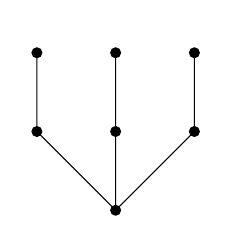
\begin{tikzpicture}
			\draw (0,0) \v -- (-1, 1) \v -- (-1,2) \v (0,0) -- (0,1) \v -- (0,2) \v (0,0) -- (1,1) \v -- (1,2) \v;
		\end{tikzpicture}
		}

		Any labeling of this graph will be not isomorphic to $G$.  For example, we could take $V'' = \{a,b,c,d,e,f,g\}$ and $E'' = \{ab, ac, ad, be, cf, dg\} $.
		\part The degree sequence for $G$ is $(3, 3, 2, 1, 1, 1 1)$.
		\part In general this should be possible: the degree sequence does not determine the graph's isomorphism class.  However, in this case, I was almost certain this was not possible.  That is, until I stumbled up this:

		\centerline{
		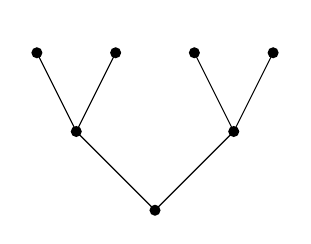
\begin{tikzpicture}
			\draw (0,0) \v -- (-1, 1) \v -- (-1.5,2) \v  (-1,1) -- (-.5,2) \v (0,0) -- (1,1) \v -- (1.5,2) \v (1,1) -- (0.5, 2) \v;
		\end{tikzpicture}
		}

		\part $G$ is a tree (there are no cycles) and as such also bipartite.
		\part Yes, all trees are planar.  You can draw them in the plane without edges crossing.
		\part The chromatic number of $G$ is 2.  It shouldn't be hard to give a 2-coloring (for example, color $a, d, e, g$ red and $b, c, f$ blue), but we know that all bipartite graphs have chromatic number 2.
		\part It is clear from the drawing that there is no Euler path, let alone an Euler circuit.  Also, since there are more than 2 vertices of odd degree, we know for sure there is no Euler path.
	\end{parts}
\end{Ans}
\begin{Ans}{9}
	  \begin{parts}
	  \part No.  The 9 triangles each contribute 3 edges, and the 6 pentagons contribute 5 edges.  This gives a total of 57, which is exactly twice the number of edges, since each edge borders exactly 2 faces.  But 57 is odd, so this is impossible.
	  \part Now adding up all the edges of all the 16 polygons gives a total of 64, meaning there would be 32 edges in the polyhedron.  We can then use Euler's formula $V - E + F = 2$ to deduce that there must be 18 vertices.
	  \part If you add up all the vertices from each polygon separately, we get a total of 64.  This is not divisible by 3, so it cannot be that each vertex belongs to exactly 3 faces.  Could they all belong to 4 faces?  That would mean there were $64/4 = 16$ vertices, but we know from Euler's formula that there must be 18 vertices.  We can write $64 = 3x + 4y$ and solve for $x$ and $y$ (as integers).  We get that there must be 10 vertices with degree 4 and 8 with degree 3. (Note the number of faces joined at a vertex is equal to its degree in graph theoretic terms.)
	  \end{parts}
  
\end{Ans}
\begin{Ans}{10}
  $K_{n,n}$ has $n^2$ edges.  The graph will have an Euler circuit when $n$ is even.  The graph will be planar only when $n < 3$.
  
\end{Ans}
\begin{Ans}{11}
  $G$ has 8 edges (since the sum of the degrees is 16).  If $G$ is planar, then it will have 4 faces (since $6 - 8 + 4 = 2$).  $G$ does not have an Euler path since there are more than 2 vertices of odd degree.
  
\end{Ans}
\begin{Ans}{12}
  $7$ colors.  Thus $K_7$ is not planar (by the contrapositive of the Four Color Theorem).
  
\end{Ans}
\begin{Ans}{13}
  The chromatic number of $K_{3,4}$ is 2, since the graph is bipartite.  You cannot say whether the graph is planar based on this coloring (the converse of the Four Color Theorem is not true).  In fact, the graph is {\em not} planar, since it contains $K_{3,3}$ as a subgraph.
  
\end{Ans}
\begin{Ans}{14}
		We have that $K_{3,4}$ has 7 vertices and 12 edges (each vertex in the group of 3 has degree 4).  Then by Euler's formula we have that $7 - 12 + f = 2$ so if the graph were planar, it would have $f = 7$ faces.  However, since the girth of the graph is 4 (there are no cycles of length 3) we get that $4f \le 2e$.  But this would mean that $28 \le 24$, a contradiction.
	
\end{Ans}
\begin{Ans}{15}
	If we drew a graph with each letter representing a vertex, and each edge connecting two letters that were consecutive in the alphabet, we would have a graph containing two vertices of degree 1 (A and Z) and the remaining 24 vertices all of degree 2 (for example, D would be adjacent to both C and E). By Brooks' theorem, this graph has chromatic number at most 2, as that is the maximal degree in the graph and the graph is not a complete graph or odd cycle. Thus only two boxes are needed.
\end{Ans}
\begin{Ans}{16}
		For all these questions, we are really coloring the vertices of a graph.  You get the graph by first drawing a planar representation of the polyhedron and then taking its planar dual: put a vertex in the center of each face (including the outside) and connect two vertices if their faces share an edge.
		\begin{parts}
			\part Since the planar dual of a dodecahedron contains a 5-wheel, it's chromatic number is at least 4.  Alternatively, suppose you could color the faces using 3 colors without any two adjacent faces colored the same.  Take any face and color it blue.  The 5 pentagons bordering this blue pentagon cannot be colored blue.  Color the first one red.  Its two neighbors (adjacent to the blue pentagon) get colored green.  The remaining 2 cannot be blue or green, but also cannot both be red since they are adjacent to each other.  Thus a 4th color is needed.
			\part The planar dual of the dodecahedron is itself a planar graph.  Thus be the 4-color theorem, it can be colored using only 4 colors without two adjacent vertices (corresponding to the faces of the polyhedron) being colored identically.
			\part The cube can be properly 3-colored.  Color the ``top'' and ``bottom'' red, the ``front'' and ``back'' blue, and the ``left'' and ``right'' green.
		\end{parts}
	
\end{Ans}
\begin{Ans}{17}
  $G$ has $13$ edges, since we need $7 - E + 8 = 2$.
  
\end{Ans}
\begin{Ans}{18}
  \begin{parts}
	 \part The graph does have an Euler path, but not an Euler circuit.  There are exactly two vertices with odd degree -- the path starts at one and ends at the other.
	 \part The graph is planar.  Even though as it is drawn edges cross, it is easy to redraw it without edges crossing.
	 \part The graph is not bipartite (there is an odd cycle), nor complete.
	 \part The chromatic number of the graph is 3.
  \end{parts}
  
\end{Ans}
\begin{Ans}{19}
  \begin{parts}
	 \part False.  For example, $K_{3,3}$ is not planar.
	 \part True.  The graph is bipartite so it is possible to divide the vertices into two groups with no edges between vertices in the same group.  Thus we can color all the vertices of one group red and the other group blue.
	 \part False.  $K_{3,3}$ has 6 vertices with degree 3, so contains no Euler path.
	 \part False.  $K_{3,3}$ again.
	 \part False.  The sum of the degrees of all vertices is even for {\em all} graphs so this property does not imply that the graph is bipartite.
  \end{parts}
  
\end{Ans}
\begin{Ans}{20}
	\begin{parts}
		\part False.  To prove this, we can give an example of a pair of graphs with the same chromatic number that are not isomorphic.  For example, $K_{3,3}$ and $K_{3,4}$ both have chromatic number 2, but are not isomorphic.
		\part False.  The previous example does not work, but you can easily draw two trees that have the same number of vertices and edges but are not isomorphic.  Since all trees have chromatic number 2, this is a counterexample.
		\part True.  If there is an isomorphism from $G_1$ to $G_2$, then we have a bijection that tells us how to match up vertices between the graph.  Any proper vertex coloring of $G_1$ will tell us how to properly color $G_2$, simply by coloring $f(v_i)$ the same color as $v_i$, for each vertex $v_i \in V$.  That is, color the vertices in $G_2$ exactly how you color the corresponding vertices in $G_1$.  Similarly, any proper vertex coloring of $G_2$ corresponds to a proper vertex coloring of $G_1$.  Thus the smallest number of colors needed to properly color $G_1$ cannot be smaller than the smallest number of colors needed to properly color $G_2$, and vice-versa, so the chromatic numbers must be equal.
	\end{parts}
\end{Ans}
\begin{Ans}{21}
	\begin{parts}
		\part Let $G$ be an arbitrary graph.  Assume $G$ is $3$-connected. Etc, etc etc.  Therefore $G$ is Hamiltonian.
		\part Let $G$ be an arbitrary graph.  Assume $G$ is not Hamiltonian.  Etc, etc, etc.  Therefore $G$ is not 3-connected.
		\part Let $G$ be an arbitrary graph.  Assume $G$ is 3-connected and also not Hamiltonian.  Etc, etc, etc.  This is a contradiction.
		\part Let $G$ be an arbitrary graph with $k$ vertices, and assume that for all graphs $H$ with fewer than $k$ vertices, if $H$ is 3-connected then $H$ is Hamiltonian.  Etc, etc, etc.  Therefore if $G$ is 3-connected, then $G$ is also Hamiltonian.
	\end{parts}
\end{Ans}
\begin{Ans}{22}
	All you would need to do is to produce a graph which is both $3$-connected and NOT Hamiltonian.  This is because the negation of $\forall G (P(G) \imp Q(G))$ is $\exists G (P(G) \wedge \neg Q(G))$.
\end{Ans}
 \protect \end {questions} \par \protect \end {document}
